%%%%%%%%%%%%%%%%%%%%%%%%%%%%%%%%%%%%%%%%%
% Beamer Presentation
% LaTeX Template
% Version 1.0 (10/11/12)
%
% This template has been downloaded from:
% http://www.LaTeXTemplates.com
%
% License:
% CC BY-NC-SA 3.0 (http://creativecommons.org/licenses/by-nc-sa/3.0/)
%
%%%%%%%%%%%%%%%%%%%%%%%%%%%%%%%%%%%%%%%%%

%----------------------------------------------------------------------------------------
%	PACKAGES AND THEMES
%----------------------------------------------------------------------------------------

\documentclass{beamer}

\mode<presentation> {

% The Beamer class comes with a number of default slide themes
% which change the colors and layouts of slides. Below this is a list
% of all the themes, uncomment each in turn to see what they look like.

%\usetheme{default}
%\usetheme{AnnArbor}
%\usetheme{Antibes}
%\usetheme{Bergen}
%\usetheme{Berkeley}
%\usetheme{Berlin}
%\usetheme{Boadilla}
%\usetheme{CambridgeUS} %Color rojo, me gusta
%\usetheme{Copenhagen} %Ta bueno
%\usetheme{Darmstadt} % Este es el 1er candidato
%\usetheme{Dresden} % Es lindo y parecido al de arriba
\usetheme{Frankfurt}
%\usetheme{Goettingen}
%\usetheme{Hannover}
%\usetheme{Ilmenau}
%\usetheme{JuanLesPins}
%\usetheme{Luebeck}
%\usetheme{Madrid}
%\usetheme{Malmoe}
%\usetheme{Marburg}
%\usetheme{Montpellier}
%\usetheme{PaloAlto}
%\usetheme{Pittsburgh}
%\usetheme{Rochester}
%\usetheme{Singapore}
%\usetheme{Szeged}
%\usetheme{Warsaw}

% As well as themes, the Beamer class has a number of color themes
% for any slide theme. Uncomment each of these in turn to see how it
% changes the colors of your current slide theme.

%\usecolortheme{albatross}
%\usecolortheme{beaver}
%\usecolortheme{beetle}
%\usecolortheme{crane}
%\usecolortheme{dolphin}
%\usecolortheme{dove}
%\usecolortheme{fly}
%\usecolortheme{lily}
%\usecolortheme{orchid}
%\usecolortheme{rose}
%\usecolortheme{seagull}
%\usecolortheme{seahorse}
%\usecolortheme{whale}
%\usecolortheme{wolverine}

%\setbeamertemplate{footline} % To remove the footer line in all slides uncomment this line
%\setbeamertemplate{footline}[page number] % To replace the footer line in all slides with a simple slide count uncomment this line

%\setbeamertemplate{navigation symbols}{} % To remove the navigation symbols from the bottom of all slides uncomment this line
}

\usepackage{graphicx} % Allows including images
\usepackage{booktabs} % Allows the use of \toprule, \midrule and \bottomrule in tables
\usepackage{listings}
%\usepackage{url}
\usepackage{hyperref}
\usepackage[spanish]{babel}
\usepackage[utf8]{inputenc}
%----------------------------------------------------------------------------------------
%	TITLE PAGE
%----------------------------------------------------------------------------------------

\title[Flujo Analógico]{Edición de Circuitos en Electric VLSI y simulación en gnucap} % The short title appears at the bottom of every slide, the full title is only on the title page

\author{Leandro Marsó} % Your name
\institute[] % Your institution as it will appear on the bottom of every slide, may be shorthand to save space
{
Córdoba\\ % Your institution for the title page
\medskip
\textit{elleandro@gmail.com} % Your email address
}
\date{\today} % Date, can be changed to a custom date

\begin{document}


\lstset{
basicstyle=\ttfamily,                   % Code font, Examples: \footnotesize, \ttfamily
frame=none,                             % A frame around the code
tabsize=2,                              % Default tab size
captionpos=b,                           % Caption-position = bottom
breaklines=false,                        % Automatic line breaking?
breakatwhitespace=false,                % Automatic breaks only at whitespace?
showspaces=false,                       % Dont make spaces visible
showtabs=false,                         % Dont make tabls visible
}

\begin{frame}
\titlepage % Print the title page as the first slide
\end{frame}

\begin{frame}
\frametitle{Contenido} % Table of contents slide, comment this block out to remove it
\tableofcontents % Throughout your presentation, if you choose to use \section{} and \subsection{} commands, these will automatically be printed on this slide as an overview of your presentation
\end{frame}

%----------------------------------------------------------------------------------------
%	PRESENTATION SLIDES
%----------------------------------------------------------------------------------------
\section{Edición de Circuitos} % Sections can be created in order to organize your presentation into discrete blocks, all sections and subsections are automatically printed in the table of contents as an overview of the talk

%------------------------------------------------
\begin{frame}
\subsection{Circuitos Esquemáticos}
\frametitle{Edición de Circuitos Esquemáticos}
\end{frame}
%------------------------------------------------
\begin{frame}
\subsubsection{Crear una librería}
\frametitle{Creación de una librería}
Creamos la librería que contendrá las celdas que vamos a diseñar:

File $\rightarrow$ New library

Y elegimos el nombre \textbf{analog}
\begin{figure}
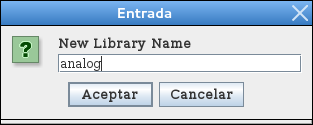
\includegraphics[width=0.35\linewidth]{figuras/edicionElectric.png}
\end{figure}
\end{frame}
%------------------------------------------------
\begin{frame}
\subsubsection{Crear una nueva celda }
\frametitle{Nueva Celda}
Creamos el esquemático de la nueva celda, con el nombre \textbf{nmosMin}: 

Cell $\rightarrow$ New Cell.
Y en View: elegimos \textbf{schematic}
\begin{figure}
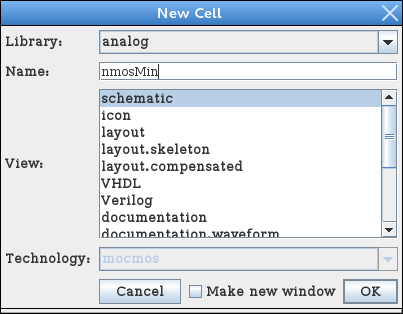
\includegraphics[width=0.45\linewidth]{figuras/edicionElectric-1.png}
\end{figure}
\end{frame}
%------------------------------------------------
\begin{frame}
\subsubsection{Instanciar un transistor}
\frametitle{Instanciar un transistor}
Vamos a la pestaña Components y seleccionamos un transistor nmos de cuatro terminales y lo instanciamos en el plano de trabajo:
\begin{figure}
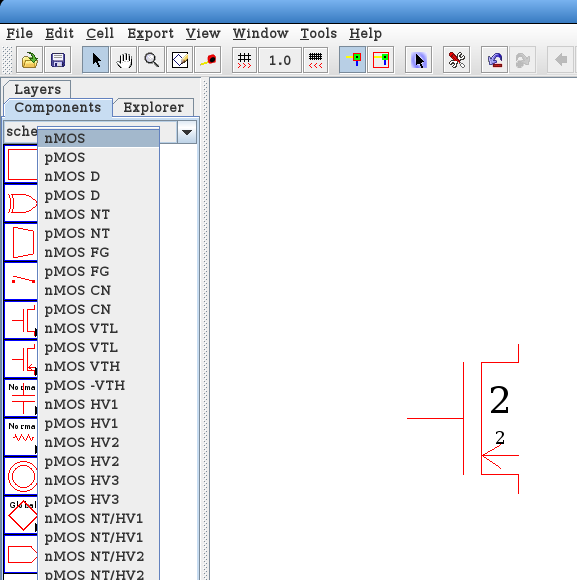
\includegraphics[width=0.5\linewidth]{figuras/edicionElectric-2b.png}
\end{figure}
\end{frame}
%------------------------------------------------
\begin{frame}
\frametitle{Editar propiedades}
Para cambiar las propiedades del transistor hacemos \textbf{Ctrl-I} y cambiamos el nombre del transistor, y dejamos el ancho y largo en 2:
\begin{figure}
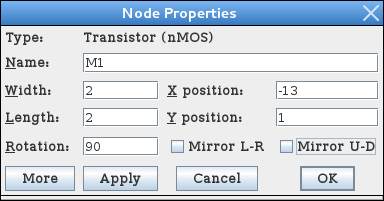
\includegraphics[width=0.5\linewidth]{figuras/edicionElectric-3.png}
\end{figure}
\end{frame}
%------------------------------------------------
\begin{frame}
\frametitle{Conectar y crear puertos}
Ahora vamos a crear puertos y exportarlos para ejemplificar el uso del simulador y una convención para los nombres.
\begin{columns}[t]
\column{.4\textwidth}
Conectamos el drenador haciendo click izquierdo sobre el mismo y luego hacemos click derecho sobre otro lado para conectar:
\begin{figure}
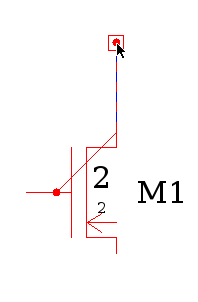
\includegraphics[width=0.5\linewidth]{figuras/edicionElectric-4.png}
\end{figure}
\column{.4\textwidth}
Nombramos el cable haciendo click izquierdo exactamente en el centro del mismo y luego \textbf{Ctrl-I} para cambiarle el nombre:
\begin{figure}
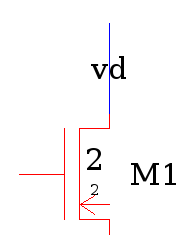
\includegraphics[width=0.5\linewidth]{figuras/edicionElectric-4b.png}
\end{figure}
\end{columns}
\end{frame}
%%%%------------------------------------------------
\begin{frame}
\subsection{Layout}
\frametitle{Creación del layout}
\end{frame}
%------------------------------------------------
\begin{frame}
\subsection{Layout Vs. Esquemático}
\frametitle{Verificación de equivalencia entre el esquemático y el layout (LVS)}
\end{frame}
%------------------------------------------------
\subsection{DRC}
\begin{frame}
\frametitle{Comprobación de errores de DRC}
\end{frame}
%------------------------------------------------
\subsection{Extracción de los parásitos}
\begin{frame}
\frametitle{Extracción de los parásitos del layout}
\end{frame}
%------------------------------------------------
\section{Simulaciones}
\subsection{Esquemático y Layout}
\begin{frame}
\frametitle{Simulación del esquemático y del layout extraído}
\end{frame}
%------------------------------------------------
\subsection{Caracterización de los transistores}
\begin{frame}
\frametitle{Caracterización de los transistores de canal N y P por medio de simulación (familia de curvas de Id/Vds)}
\end{frame}
%------------------------------------------------
\subsection{Simulaciones de punto de operación}
\begin{frame}
\frametitle{Simulaciones de punto de operación}
\end{frame}
%------------------------------------------------
\subsection{Análisis AC}
\begin{frame}
\frametitle{Análisis AC}
\end{frame}
%------------------------------------------------
\subsection{Régimen transitorio}
\begin{frame}
\frametitle{Régimen transitorio}
\end{frame}
%------------------------------------------------
\subsection{Transformada de Fourier}
\begin{frame}
\frametitle{Transformada de Fourier}
\end{frame}
%------------------------------------------------
\subsection{Alternativas de Interacción con circuitos digitales}
\begin{frame}
\frametitle{Alternativas de Interacción con circuitos digitales}
\end{frame}
%------------------------------------------------

\begin{frame}
\Huge{\centerline{Fin}}
\end{frame}

%----------------------------------------------------------------------------------------

\end{document} 
